\documentclass[a4paper, 10pt]{article}

%Internal Packages
\usepackage[utf8]{inputenc}
\usepackage[french]{babel}
\usepackage[T1]{fontenc}
\usepackage{graphicx}
\usepackage{hyperref}       % Pour les liens hypertextes

%Variables
\title{Rapport de projet : CoreWar}
\author{Amand Henry\and{}Théo Sicot\and{}Etienne Bossu\and{}Tom Rousée}
\date{\today{}}

%Document
\begin{document}
    \maketitle{}
    \newpage{}
    \tableofcontents{}
    \newpage{}

    % Introduction
    \begin{section}{Introduction} \label{sec:introduction}
        \par
            Le \textbf{Corewar} est un jeu de programmation créé en 1984 dans les universités américaines où deux programmes sont opposés pour prendre le contrôle d'une machine virtuelle appelée \textbf{MARS} (Memory Array Redcode Simulator). Ces programmes sont écrits dans un langage proche de l'assembleur appelé \textbf{RedCode}. Les programmes, appelés "Guerriers", ont pour objectif d'être les derniers à s'exécuter en faisant se terminer toutes les instances du programme adverse.
            \medskip
        \par
            Au début les joueurs concevaient leurs programmes par eux mêmes mais avec la popularisation des \textbf{algorithmes génétiques}, beaucoup utilisent l'ordinateur pour essaier de trouver les meilleurs programmes possible et gagner la partie.
            \medskip
        \par
            Ce projet était principalement tourné vers la création d'un algorithme génétique, cependant pour pouvoir le tester, il fallait créer un jeu de CoreWar complet. C'est donc ce que nous avons fait. Nous avons créé un jeu de CoreWar complet avec une machine MARS, un RedCode, un algorithme génétique et une interface graphique pour visualiser les parties.
            \medskip
        \par
            Après avoir présenté les objectifs du projet, nous allons détailler le RedCode, la machine MARS, l'algorithme génétique et l'interface graphique que nous avons créé. Nous présenterons ensuite les résultats obtenus et conclurons sur ce que nous avons appris et les perspectives d'évolution que nous pourrions mettre en place.
            \bigskip

        \begin{subsection}{Objectifs}
            \par
                L'objectif de ce projet était de créer un jeu de CoreWar complet. Pour cela nous avons dû identifier les points principaux qui composent notre projet et les implémenter. Nous avons donc décidé de découper notre projet en plusieurs parties :
                \smallskip
                \begin{enumerate}
                    \item Le RedCode
                    \item La machine MARS
                    \item Un algorithme génétique pour créer des guerriers
                    \item Une interface graphique pour afficher le déroulement des parties
                \end{enumerate}
                \medskip
                Nous avions pour la réalisation de ce projet un peu plus de 3 mois. Durée de temps appropriée car elle nous a permis de bien réfléchir aux détails de la création du jeu et de le réaliser dans les temps sans avoir a délaisser les autres cours.
                \bigskip
        \end{subsection}
    \end{section}
    

    \begin{section}{Le RedCode : Détails du Langage}
        \par
            Le \textbf{RedCode} est un langage proche de l'assembleur, uniquement utilisé par les joueurs de CoreWar et qui permet de programmer les guerriers. On utilise ce langage car par défaut il n'est pas compris par les ordinateurs. Cela évite que des personnes mal-intentionnées, ou simplement des erreurs, créent des bugs sur les pc des joueurs comme il n'y a pas risque qu'ils s'échappent de la machine MARS. Au fur et à mesure des années ce langage a évolué avec l'ajout de nouvelles instructions mais pour ce projet nous utilserons une de ses premières versions : la norme icw88 (créee een 1988). 
            
            Dans cette version, le Redcode se compose de 11 instructions. Les instructions sont des commandes qui permettent de déplacer les guerriers, de modifier la mémoire, de sauter des instructions, etc. Les opérandes sont quant à eux un couple valeur-mode qui associe un entier et le mode d'adressage de cette valeur (Direct, Indirect, Immédiat et Pre-Decrement).
            \bigskip \newline
                \textit{Voici les différentes instructions et leurs effets :}
            \bigskip

            \begin{tabular}{|c|p{8cm}|}
                \hline
                    \textbf{Instruction} & \textbf{Description} \\
                \hline
                    DAT A B & Supprime le processus en cours d'exécution de la file d'attente des processus \\
                \hline
                    MOV A B & Déplace A dans B \\
                \hline
                    ADD A B & Ajoute A à B \\
                \hline
                    SUB A B & Soustrait A à B \\
                \hline
                    JMP A B & Saute à A \\
                \hline
                    JMZ A B & Saute à A si B est égal 0\\
                \hline
                    JMN A B & Saute à A si B est différent de 0 \\
                \hline
                    CMP A B & Si A est égal à B, ignore l'instruction suivante\\
                \hline
                    SLT A B & Si A est inférieur à B, ignore l'instruction suivante\\
                \hline
                    DJN A B & Décrémente B; Si B est différent de 0, saute à A \\
                \hline
                    SPL A B & Place A dans la file d'attente des processus \\
                \hline
        \end{tabular}

        \bigskip
        Ensuite, pour définir sur quelle cellule l'instruction va s'éxécuter on retrouve 4 modes d'adressage différents. Ils sont représentés par des symboles et sont associés aux valeur A et B pour former des \textbf{Operandes}.
        \bigskip \newline
            \textit{Voici les différents modes d'adressage et leurs effets :}
        \bigskip

        \begin{tabular}{|c|p{8cm}|}
            \hline
                \textbf{Mode} & \textbf{Description} \\
            \hline
                Direct & L'opérande est une adresse mémoire vers une autre cellule \\
            \hline
                Indirect & L'opérande est une adresse mémoire vers une autre adresse (Comme si on faisait 2 Direct) \\
            \hline
                Immédiat & L'opérande est une valeur \\
            \hline
                Pre-Decrement & Similaire à l'indirect mais on fait -1 sur la deuxième adresse avant d'aller chercher la cellule \\
            \hline
        \end{tabular}

        \bigskip
        Afin de pouvoir créer des guerriers et réaliser notre projet, il est nécessaire de bien comprendre le RedCode, ses instructions et modes d'adressage. Nos premières séances furent donc dédiées a la compréhension du fonctionnement de ces derniers. Une fois compris, nous avons pu créer notre machine MARS qui interprète ces instructions et les exécute.
        \bigskip
    \end{section}




    \begin{section}{Machine MARS : Mémoire et Déroulement de la partie}
        \par
            La \textbf{machine MARS} est la pièce maitresse des parties de CoreWar. C'est la machine virtuelle dans laquelle les guerriers vont s'exécuter. Elle gère la mémoire, interprète le RedCode et est responsable du déroulement des parties, sans elle pas de projet c'est donc par là que nous avons commencé notre travail. 
            \medskip
        
        \begin{subsection}{Mémoire}
            
            \par
                Une des problèmatiques de cette partie était la \textbf{représentation de la mémoire}.
                Nous avons choisi d'utiliser une \textbf{liste doublement chainée} car la mémoire devait être circulaire et il facile de réaliser ce type de mémoire avec cette structure de données.
                \smallskip
            \par
                Dans cette liste chainée chaque cellule contient \textbf{une instruction et deux Operandes}. Pour rappel, les instructions sont les commandes que les guerriers vont exécuter et les Operandes contiennent les informations sur la méthode a appliquer pour exécuter l'instruction. 
                \medskip

                \begin{figure}
                    \includegraphics[width=10cm]{img/umlMemoire.png}\label{fig:umlMemoire}
                    \caption{Diagramme UML de la mémoire}
                \end{figure}
        \end{subsection}
        
        \begin{subsection}{Déroulement d'une partie}
            \par
                La machine MARS doit aussi gérer le déroulement de la partie. L'idée est que chaque guerrier exécute chacun à son tour une instruction. Pour cela elle a aussi à sa disposition une liste des instructions à exécuter, qui est en fait une liste de certaines cellules de la mémoire (celles dans lesquelles un guerrier à une opération en cours). Cela permet de facilement déterminer quel guerrier doit jouer et de lui faire exécuter son instruction au bon moment.
            \par
                //TODO : Développer sur la process Queue / Différence Programme, instruction et processus ? Illustrer la process queue ?
        \end{subsection}
        \bigskip
    \end{section}



    \begin{section}{Algorithme Génétique}
        \par
            Après avoir créer la machine MARS nous avons pu développer l'algorithme génétique. L'objectif étant d'avoir un algorithme qui crée des programmes en RedCode qui sont des meilleurs guerriers que les précédent. On peut dissocier le développement de cet algorithme en deux grandes parties : Le Fonctionnement de l'algo en lui même et ensuite les différentes méthodes afin de l'entrainer efficacement.
            \medskip

        \begin{subsection}{Fonctionnement}

            \begin{subsubsection}{Création de guerriers aléatoires : les seeds}
                \sloppypar
                    Nous avons opté pour un algorithme génétique dans lequel on retrouve une grande partie d'aléatoire. Cela permet idéalement de ne pas rester bloqué sur certains programmes et d'avoir un guerrier qui est bon contre la majeure partie de ses adversaires en explorant un maximum de possibilités.
                    \smallskip
                \par
                    Pour cela il a d'abord fallu pouvoir générer un guerrier aléatoirement. Nous avons alors travailler sur un système de génération de \textbf{seeds} aléatoires. Ces seeds sont des nombres générés aléatoirement que l'on peut convertir en une ligne de RedCode. 
                    \medskip
                \par
                    \textit{\textbf{Exemple :} la ligne de RedCode "ADD @10, <5" est représenté par la ligne 02101005, 02 étant le code de l'instruction ADD, le premier 10 les modes d'adressage, puis enfin 10 et 05 les valeurs de A et B.}
                    \bigskip
                \par
                    Une fois que l'on a généré une ligne aléatoirement il suffit tout simplement de la placer dans une \textbf{"seedline"} un ArrayList de Seed qui nous permet de représenter un guerrier. On peut alors créer un guerrier aléatoirement a partir de rien. Et c'est en générant plusieurs de ces guerriers que l'on peut créer une population.
                    \bigskip
            \end{subsubsection}

            \begin{subsubsection}{L'amélioration des populations}
                \par
                    Une fois que l'on a généré une population il faut pouvoir l'améliorer. Pour ce faire nous avons travaillé sur un système de reproduction et de mutation.
                    \medskip
                \par
                    La \textbf{reproduction} consiste à prendre deux guerriers de la population et à les croiser pour créer un nouveau guerrier. Pour cela on prend une partie de la seedline d'un guerrier et on la remplace par une partie de la seedline de l'autre guerrier. Cela permet de créer un nouveau guerrier qui a des caractéristiques des deux guerriers de départ. On choisit un pivot aléatoirement dans la plus petite graine et on échange les parties de la seedline avant ou après ce pivot (décidé a Pile ou Face).
                    \medskip
                \par
                    Afin que le système de reproduction soit efficace nous avons choisi de faire en sorte que le guerrier le plus performant de la population se reproduise avec tout les autres guerriers. Cela permet de garder les caractéristiques du guerrier le plus performant et de les diffuser dans toute la population afin d'en obtenir une nouvelle.
                    \medskip
                \par
                    Pour déterminer le guerrier le plus performant il a fallu réfléchir a des méthodes de scoring. Nous avons choisi de faire s'affronter les guerriers deux par deux et de compter le nombre de victoires de chacun. Le guerrier qui a le plus de victoires est alors le guerrier le plus performant. Aussi un guerrier qui s'est suicidé dans les 32 premiers cycles ne rapporte pas de point au gagnant mais en fait perdre un. Cela permet de pénaliser les guerriers qui se suicident trop rapidement sans récompenser celui qui gagne a cause d'eux. 
                    \medskip
                \par
                    La \textbf{mutation} est un autre moyen d'améliorer les guerriers. Elle consiste à prendre un guerrier et à changer une partie de sa seedline aléatoirement. Cela permet de créer des guerriers qui sont différents de ceux de la population et qui peuvent être meilleurs.
                    \medskip
                \par
                    Pour que la mutation soit efficace il a fallu déterminer un taux de mutation. A chaque reproduction le guerrier obtenu a une chance sur 3 de muter. Cela permet de ne pas trop modifier les guerriers et de ne pas perdre les caractéristiques des guerriers de départ.
                    \medskip
                \par
                    4 types de mutations ont été implémentées : 
                    \begin{itemize}
                        \item \textbf{Modified} : Modifie une des 4 données de la seed aléatoirement (Instruction, Modes, Valeur de A, Valeur de B), si c'est une instruction on change aussi le mode d'adressage en fonction pour éviter les erreurs.
                        \item \textbf{Additional} : On ajoute une ligne de RedCode aléatoire dans le guerrier.
                        \item \textbf{Removal} : On supprime une ligne de RedCode aléatoire du guerrier.
                        \item \textbf{Swap} : On intervertit deux lignes du guerrier entre elles aléatoirement.
                    \end{itemize}
                    \bigskip
                \par
                    Enfin, pour que l'algorithme génétique soit efficace il a fallu déterminer un nombre de générations. Nous avons choisi de faire 100 . Cela permet de bien faire évoluer les guerriers et de ne pas rester bloqué sur des guerriers qui ne sont pas performants.
                    \bigskip

            \end{subsubsection}
        \end{subsection}

        \begin{subsection}{Entrainement}
            \par
                Une fois notre algorithme génétique créé il a fallu l'entrainer. Pour cela nous avons du générer une population aléatoire puis y faire s'affronter les guerriers et les faire évoluer en conséquence. Cette opération doit être répété plusieurs miliers de fois pour que les guerriers soient performants. Afin de réduire le temps d'entrainement nous avons fait évoluer nos méthodes et développé 3 façons d'entrainer nos guerriers et de vérifier que l'algo fonctionne ont été implémentées.

                \begin{subsubsection}{Le CheatCode DAT}
                    \par
                        Il nous fallait d'abord une méthode très rapide et très simple qui nous permettrait de vérifier que l'algorithme marche. Pour cela nous avons décidé d'une méthode très simple : le CheatCode.
                        \medskip
                    \par
                        Le CheatCode est une ligne qui permet de gagner la partie en un seul coup. En effet nous avions décidé que si un guerrier avait une ligne dont l'instruction était DAT alors il gagnait automatiquement la partie. Cela permettait de vérifier que l'algorithme marchait et que les guerriers trouveraient cette ligne et la garderaient dans les générations suivantes.
                        \medskip
                    \par
                        Au départ lorsque l'on générait une population aléatoire il y avait forcément très peu de guerriers qui contenaient une instruction DAT mais après a peine quelques générations on pouvait voir que les guerriers gardaient cette instruction et que la population était de plus en plus performante. L'algorithme fonctionnait donc bien !
                        \bigskip
                \end{subsubsection}

                \begin{subsubsection}{Entrainement d'une population aléatoire}
                    \par
                        Une fois que l'on a vérifier que l'algorithme marche il faut donc trouver un moyen d'entrainer les guerriers réellement. Et oui, dans une partie de CoreWar pas de Cheatcode. La première méthode qui nous est venue en tête était de générer une population aléatoire et de faire s'affronter chacun des guerriers de cette population. Le guerrier qui avait le plus de victoire était le plus performant et on pouvait alors le faire se reproduire avec les autres guerriers de la population.
                        \medskip
                    \par
                        Cette méthode est celle qui nous permettrait d'avoir le guerrier le plus précis et meilleur contre le plus d'adversaire. Cependant elle est aussi la plus longue. 100 guerriers qui participent chacun a 100 combats a chaque génération, c'est quand même 10000 combats a répéter plusieurs centaines si ce n'est milliers de fois. C'est quand nous avons pris conscience du temps que cela allait prendre de générer des programmes performants que nous avons décidé de mettre en place l'utilisation des \textbf{threads} pour accélérer le processus. En effet, grâce aux threads on peut faire se dérouler plusieurs combats simulatanément en affectant une machine par thread et donc réduire drastiquement le temps nécessaire pour l'entrainement. Mais le temps restant long nous avons également mis en place un moyen de sauvegarder la progression. On exporte la dernière population et ses scores dans des fichiers binaires et on les importe lorsque l'on relance le programme. Cela permet de ne pas perdre de temps a reentrainer une population déjà entrainée.
                        \medskip
                    \par
                        Une fois le temps d'entrainement réduit nous avons aussi eu besoin de moyen de visualiser l'amélioration de nos guerriers. Pour cela nous avons décidé de générer des graphiques nous affichant l'évolution des scores de nos guerriers.
                        \medskip
                    \par
                        \textit{Cependant voici les graphiques que nous avons obtenu :}
                        \medskip
                    \par
                        \includegraphics[width=10cm]{img/graphique1.png}
                        \bigskip
                    \par
                        \includegraphics[width=10cm]{img/graphique2.png}
                        \bigskip
                    \par
                        Comme on peut les voir les courbes de ces graphiques ne montrent pas d'évolution probante. Cela est du au fait que avec notre méthode d'affichage et d'entrainement nous n'avons pas un référentiel de comparaison. En effet, un programme qui a un score de 120 a la première génération n'est pas forcément meilleur qu'un programme qui a un score de 100 a la 10ème génération. Un a battu des programmes plus faibles que l'autre. C'est pour cela qu'il nous fallait revoir notre méthode de scoring et d'entrainement pour avoir des résultats plus pertinants a vous montrer.
                \end{subsubsection}    

                \begin{subsubsection}{Le Challenger}
                    \par
                        Pour avoir un référentiel de comparaison nous avons décidé de créer un guerrier qui serait notre référence. Ce guerrier, appelé le \textbf{Challenger}, est un guerrier qui a été créé par un humain et qui est considéré par la communauté des joueurs de CoreWar comme performant. Il est donc notre référence pour savoir si nos guerriers sont performants ou non.
                        \medskip
                    \par
                        Chaque guerrier de notre population est donc confronté au Challenger et on peut alors voir si il est performant ou non. Cela permet de savoir si notre algorithme génétique est efficace et si nos guerriers sont de plus performants.
                        \medskip
                    \par
                        Cependant si on ne fait seulement des combats contre le Challenger et que l'on ne fait pas s'affronter les guerriers entre eux on n'obtiendrait un programme uniquement performant face au Challenger avec très peu d'adaptabilité face à d'autres guerriers. Les guerriers ont donc deux scores : un score face au Challenger et un score face aux autres guerriers de la population. Cela permet de savoir si un guerrier est performant ou non.
                        \medskip
                    \par
                        Le score du challenger est celui que l'on affiche dans les graphiques. Cela permet de voir l'évolution de nos guerriers face à un guerrier performant et de savoir si notre algorithme génétique est efficace. L'autre score sert toujours a déterminer le guerrier le plus performant de la population pour l'amélioration de cette dernière.
                        \bigskip
                    \par 
                        \textit{Voici les graphiques que nous avons obtenu avec cette méthode :}
                        \medskip
                    \par
                        \includegraphics[width=10cm]{img/graphique3.png}
                        \bigskip
                    \par
                        On voit sur ce graphique que la tendance globale est descendante c'est donc bien que les algorithmes s'améliore face au Challenger. Cependant on voit aussi que les scores sont très variables. Cela est du au fait qu'une population dans laquelle la plupart des programmes se suicident ne donnent que très peu de point au Challenger car pour rappel, si un programme se suicide on ne donne pas de point au gagnant, on en enlève un au perdant. L'idée est de voir la tendance des pics de score qui sont ceux d'une génération ou peu, voir aucun programme ne se suicident. On voit bien qu'ils descendent c'est donc bien que le Challenger perd de plus en plus de combat et est donc confronté a des algorithmes de plus en plus performants.
                \end{subsubsection} 
                
        \end{subsection}
    \end{section}

    \begin{section}{Interface Graphique}
        \par
            L'interface a été faite avec le package \textbf{swing}, déjà inclus dans java. Elle permet de visualiser une partie et ne se lance que si on lui demande. On ralentit le temps entre deux instructions quand elle est appelée sinon la partie se termine trop rapidement pour que ce soit lisible. Elle transforme la mémoire en une grille. Cette grille s'adapte à toute les tailles de mémoire pour d'éventuelles parties sur une mémoire a taille réduite. Elle est composée de cases qui peuvent être de 3 couleurs différentes : Bleu, Rouge et Noir. (le Bleu et le Rouge pour chacun des guerriers et le Noir pour les cases qui n'appartiennent encore a personne).
            \bigskip
        
            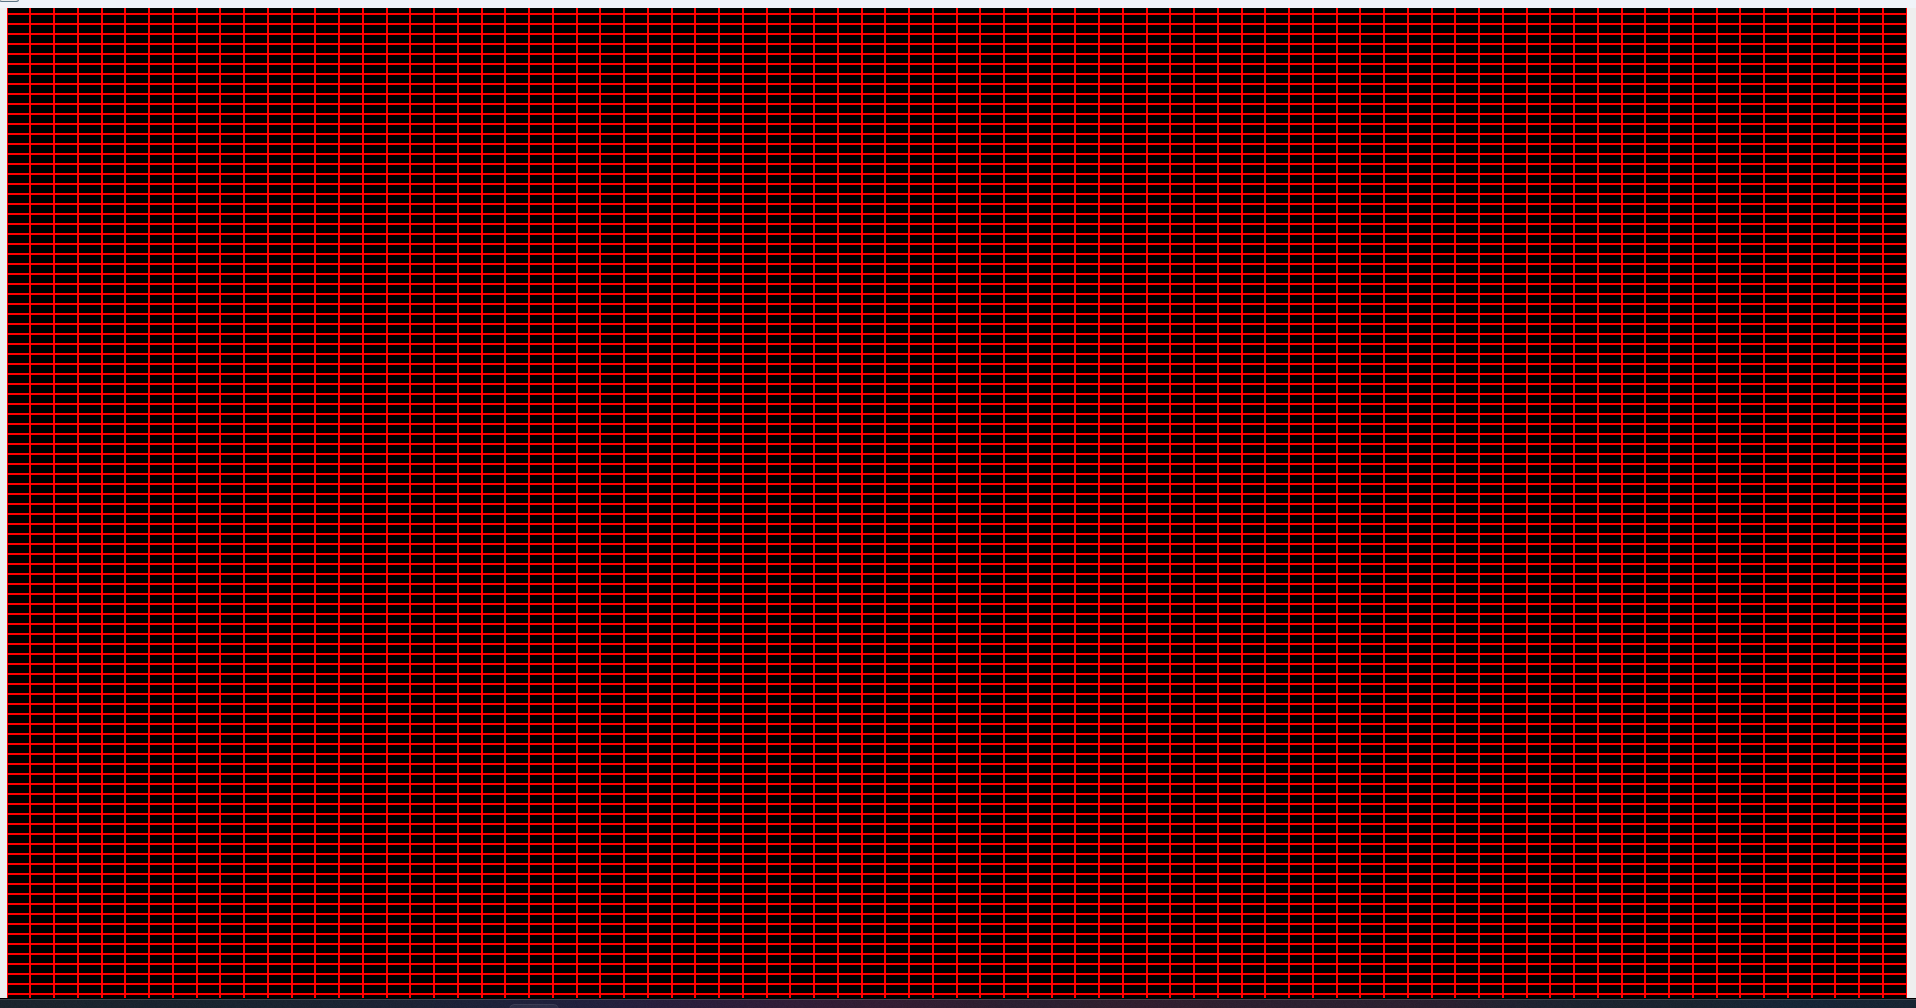
\includegraphics[width=10cm]{img/grille_interface.png}\newline
            \textit{La grille de 8000 cases, taille la plus courante pour les parties de CoreWar.}
            \bigskip

        \par
            Pour l'affichage final on efface les bordures pour afficher uniquement les couleurs et evider de surcharger l'interface.
            \bigskip

            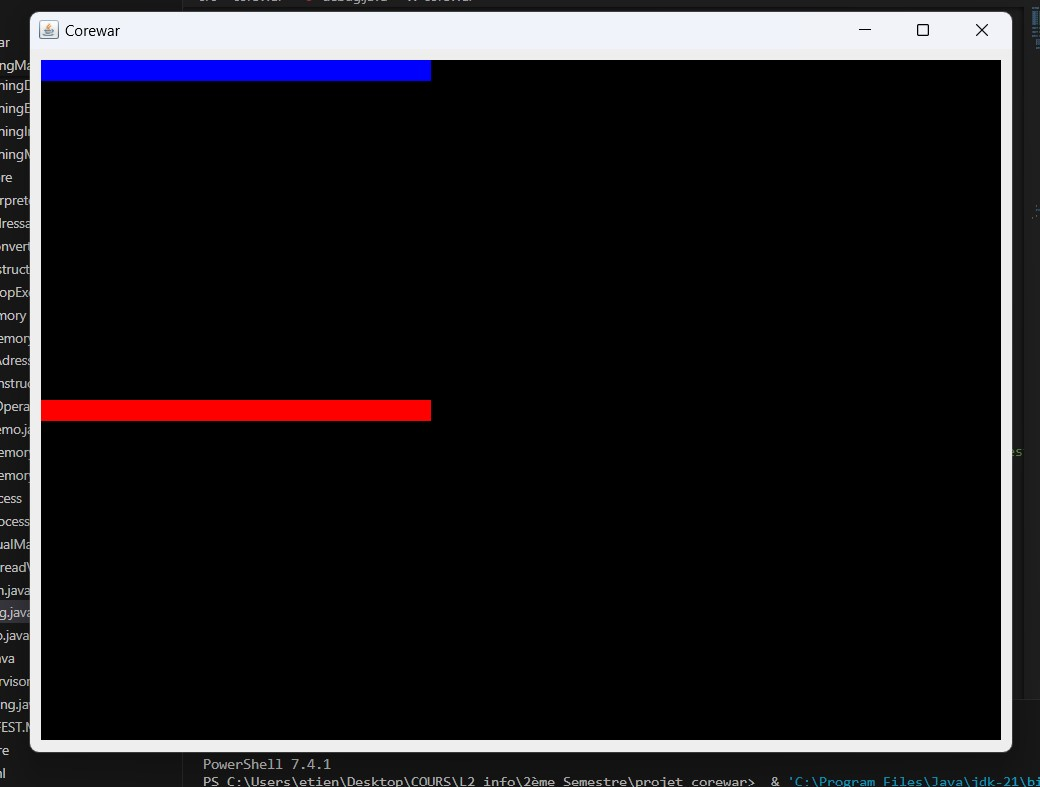
\includegraphics[width=10cm]{img/display.jpg}\newline
            \textit{Affichage final de l'interface graphique. Sans les bordures durant une partie.}
            \bigskip
        
        \par
            Pour actualiser l'affichage plusieurs méthodes ont été créées. Au départ la méthode consistait a prendre une nouvelle grille et à remplacer l'ancienne par la nouvelle. Mais cela ralentissait énormément l'affichage. Nous avons donc décidé de créer une méthode qui actualise uniquement les cases qui ont changé de couleur. Cela a permis d'optimiser l'affichage et de ne pas ralentir le jeu.
            Pour ce faire l'utilisation d'un GridBagLayout plutôt qu'un GridLayout simple a été nécessaire et il a fallu recréer l'interface. Dorénavant chaque case est gérée comme un élément indépendant et peut être actualisée indépendamment des autres.
    \end{section}

    \begin{section}{Conclusion : Résultats et Perspectives d'évolutions}\label{sec:resultats}
        \par
            Les résultats obtenus sont plutôt satisfaisants. Nous avons réussi à créer un jeu de CoreWar complet avec une machine MARS, un RedCode, un algorithme génétique et une interface graphique. Nous avons pu voir que l'algorithme génétique fonctionnait et que les guerriers créés étaient performants.
            \medskip
        \par
            Cependant il reste des points à améliorer. L'algorithme génétique pourrait être amélioré pour être plus performant. Une perspective d'évolution serait de faire en sorte que le challenger soit une population test et non un guerrier unique. Cela permettrait de voir si nos guerriers sont performants face à une population plus clairement. Il faudrait aussi améliorer l'affichage des graphiques et de l'interface pour qu'ils soient plus clairs et plus précis.
            Il pourrait être intéressant aussi de tester de nouveaux types de mutations et d'algorithme pour voir si certains sont plus performants que d'autres.
            \medskip
        \par
            Une de nos principales contraintes fut aussi la contrainte matérielles. En effet générer des milliers de population prend du temps et nécessite d'avoir un ordinateur suffisament puissant a sa disposition pour le laisser tourner et générer un maximum de programme en un minimum de temps. Il serait donc intéressant de voir si l'on atteint un guerrier ultime, meilleur que tout les autres, après un certain temps de génération. Cela permettrait d'avoir une idée plus claire de ce que l'on peut obtenir avec notre algorithme génétique.
            \medskip
        \par
            Enfin, il serait intéressant de tester notre algorithme génétique sur d'autres jeux de programmation pour voir si il est performant et si il peut être utilisé pour créer des programmes performants dans d'autres domaines.
        \par
            Ces possibilités d'amélioration ne réduit en rien notre satisfaction d'avoir réussi à créer un jeu de Corewar complet et de voir que notre algorithme génétique fonctionne. Nous avons appris beaucoup de choses durant ce projet, avons appris de nouvelles manières de travailler et de nouvelles notions de programmation. C'est donc un projet que nous avons beaucoup apprécié et qui nous a permis de progresser.
    \end{section}

    % Références
    \bibliographystyle{plain}
    \bibliography{references}
    
\end{document}